\documentclass{sig-alternate}

\begin{document}
\conferenceinfo{UWCSE503}{'10 Seattle, WA USA}

\title{JavaGrok: Automatic Inference of Documentation for Under-documented Code}

\numberofauthors{1} 
\author{
\alignauthor
Colin S. Gordon, Reto Conconi, Gilbert Bernstein, Michael Bayne\\
       \affaddr{University of Washington}\\
       \affaddr{Seattle, WA USA}\\
       \email{\{csgordon,conconir,gilbo,mdb\}@cs.washington.edu}
}

\maketitle
\begin{abstract}
Modern software development increasingly involves the use of third party
libraries. Developers now routinely locate and learn the APIs of myriad
libraries in the course of a single software development project. This process
is made more difficult by the fact that many libraries are poorly documented.
The developer often has to read the library source code or resort to trial and
error to determine how to correctly use the library. These methods of learning
about the library are time consuming and error prone.

We present a method to automatically augment library API documentation with invariants
inferred by a variety of static analyses. These include argument nullability,
argument and receiver mutation, argument leaking and capturing, and conditions
that will cause exceptions to be thrown.
\end{abstract}

% A category with the (minimum) three required fields
\category{H.4}{Information Systems Applications}{Miscellaneous}
%A category including the fourth, optional field follows...
\category{D.2.8}{Software Engineering}{Metrics}[complexity measures, performance measures]

\terms{Delphi theory}

\keywords{ACM proceedings, \LaTeX, text tagging}

\section{Introduction}

Despite their best intentions, many developers routinely fail to provide
adequate or any documentation for the code they write.  Whether because of poor
practice, lack of time or a sincere belief on the part of programmers that their
code will soon be thrown away, much code in regular use remains undocumented.
New developers join the team, the code is handed off to another group, or
perhaps even posted publicly on the Internet.  By various means, this code
finds its way into the hands of programmers who---having been assured that this
code will save them weeks of effort---now face a thoroughly unenviable task:
grok a lump of un(der)documented code and learn its interface well enough
to solve their original problem.

We believe it would be useful to have a tool that could generate partial
documentation of at least simple properties.

The prototype tool we describe here, JavaGrok, seeks to do just this.  By
applying static analyses to infer properties of library source code and then
translating the results into human readable form, we are able to
automatically construct or augment Javadoc documentation.
Using this tool, we
consider the hypothesis that a significant amount of user pain and frustration
with un(der)documented libraries is due to confusion about
properties discoverable via static analyses. We consider analyses for argument nullability,
reference leaking and capturing, and exceptional conditions.
Here, we focus on confusions about formal properties
rather than conceptual
or higher level confusions about the proper way to use a library.

Although there has been previous work on automatic
documentation~\cite{autodoc}, we perform the first user study
focused on whether automatically generated documentation is helpful for program
understanding.  By contrast, previous work~\cite{autodoc, Nimmer2002} has
evaluated the benefit of program analyses to users in verification tasks or the
accuracy of generated annotations relative to exemplar documentation.
We believe that determining whether automatically generated documentation helps
developers understand code is the logical next step, and more relevant to practice.

Our user study compares developers'
experience using a poorly documented library with and without JavaGrok
annotations.  We measured how often users were confused and how they resolved their confusion.  We also collected qualitative exit
questionnaires.  Unfortunately, we found no evidence that JavaGrok had
significant impact, positive or negative on the user experience.  We discuss
reasons why our evaluation was not conclusive and possible alternative
evaluations later.


\section{Technical Approach}
To infer information about Java code we use existing Java inference tools and 
combine their output. Additionally we have our own framework which allows us to
implement our own analysis. 

Most inference tools available put annotations into 
the Java class files. So does our own framework. To get the inferred information
back into the source files we use the annotation file utilities \cite{AFU} 
(TODO: How to cite a website???). 
These consist of several tools. One allows to extract annotations
from the class files. Thereby the information gets stored in an external file.
Javarifier - one of the tools which we use - directly supports to generate those
external annotation files. In a next step we use another annotation file utility which
merges the source files with the corresponding annotation files.

\begin{figure}
\centering
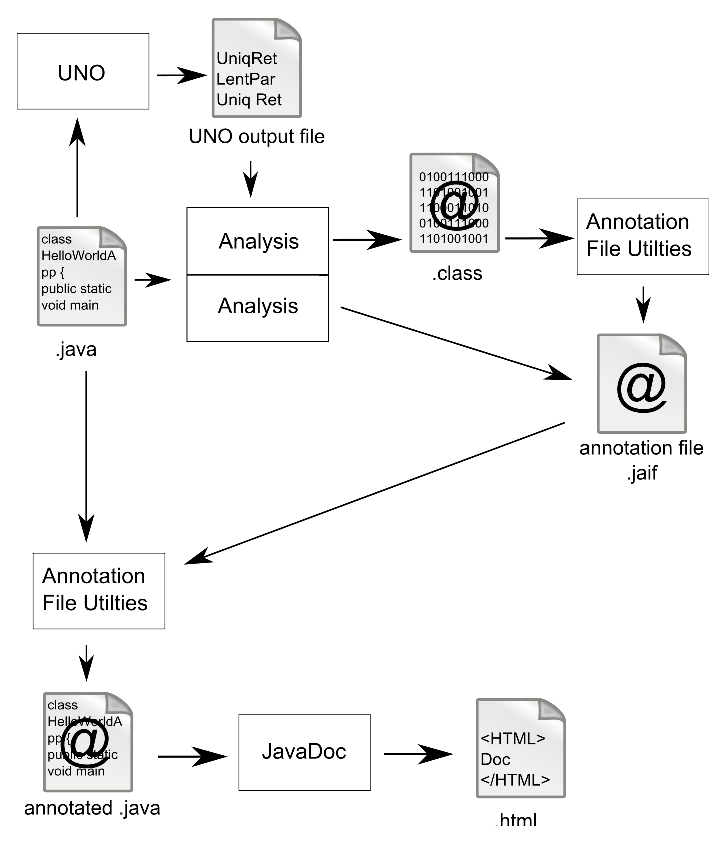
\psfig{file=figures/technicalApproach/technicalApproach.eps, width=2.1in}
\caption{Toolchain}
\end{figure}

\subsection{Analysis Framework}

To implement our own analysis tools we use the current version of the Java 7 compiler.
This allows us to use it's plugin architecture to write our own analyzers. From within
a Java compiler plugin we can access the compiler's abstract syntax tree and we can emit 
annotation to the class files. As described above those annotation will get extracted 
with the annotation file utilities.


\section{Evaluation} \label{sec:Evaluation}
We performed a small experiment wherein developers were given a third party
library with documentation and a set of programming tasks. They were asked to report on certain
events that occurred while completing the tasks. We specifically focused on
when the developer had questions about how to correctly use the library, and
considered four cases: a) the question was answered by our annotations, b) the
question was answered by the existing library documentation, c) the question
was answered by reading the library source code, and d) the question was not
answered. We also asked the developers to note any time they were surprised by
the library's behavior.

Our hypothesis was that by augmenting library documentation with inferred
properties, we would decrease the frequency with which developers needed to
refer to the library source code to answer questions. This would show up as a
non-zero incidence of questions being answered by annotations and a
corresponding decrease in the questions that were answered by reading source
code. We also hypothesized that our annotations may have resulted in a
reduction in surprise at library behavior, and would not increase the incidence
of surprise.

\begin{figure*}
\centering
\begin{tabular}{ l | r r r r | r }
 & \multicolumn{4}{| c | }{Question answered by:} & \\
Developer & Annotations & Docs & Source & Unanswered & Surprised \\
\hline
Dev 1 & 0 & 14 & 0 & 1 & 0 \\
Dev 2 & 1 &  5 & 2 & 1 & 0 \\
Dev 3 & 1 &  3 & 0 & 0 & 0 \\
Dev 4 & 1 &  6 & 1 & 1 & 0 \\
\hline
\textit{Experiment} & 3 & 28 & 3 & 3 & 0 \\
\hline
Dev 5 & - &  4 & 0 & 0 & 0 \\
Dev 6 & - & 13 & 2 & 3 & 1 \\
Dev 7 & - & 10 & 0 & 2 & 0 \\
Dev 8 & - &  7 & 1 & 2 & 1 \\
\hline
\textit{Control} & - & 34 & 3 & 7 & 2 \\
\hline
\end{tabular}
\caption{Experiment Results}
\label{fig:exp_results}
\end{figure*}

\medskip
\subsection{Experiment Design}
The experiment involved two groups of four developers each, all of whom were
University of Washington computer science graduate students. The developers
were given a set of programming tasks involving the creation of simple
interactive animations. They were supplied with the Nenya~\cite{nenya} graphics
and animation library to use to complete those tasks. None of the developers had
previously seen or used the library. The experimental group was provided with
augmented documentation and source code for the library, and the control group
was provided with original, unmodified documentation and source code.

There were four tasks that were designed to consume at least one
hour. Developers were told that they were free to leave after one hour, even if
they had not completed all of the tasks.

The members of each group were provided with the Eclipse IDE, configured to
provide ready access to the appropriate documentation and source code. As the
subjects' experience with the Eclipse IDE was quite varied, they were shown how
to access both the library documentation and source code. The aim was to reduce
the likelihood that differing familiarity with the IDE would influence their
decision to inspect the documentation or source.

The subjects were instructed to first check the documentation when they
encountered a question about correct usage of the library, then to consult the
source code only if their question was not answered to their satisfaction by
the documentation. Finally they were asked to record the outcome of each event.
The experimenter could record a question as being resolved by ``annotations'',
``documentation'', ``source code'' and ``not resolved''. The control group had
only the latter three choices as they had unaugmented documentation.

We also instructed subjects to complete a short survey after finishing the
experimental tasks. The results of this survey were not intended to directly
validate or refute our hypothesis, but to help us to gauge other aspects of the
work, better understand ambiguous results, and to direct future work. Data from
the survey are mentioned in the discussion below. The results of our experiment
are shown in Figure ~\ref{fig:exp_results}.

\subsection{Discussion}
For our small test group, a striking difference between the control and
experimental groups would have been necessary to support our hypothesis.  The
results had no such strong
trends, rather they were inconclusive.  Our sample size of developers was not
large enough to be statistically significant, but the developer surveys exhibit
a mixture of both positive and negative trends.

Most developer complaints from both the experimental and control groups were
about the high-level usage model of the library being unclear.  This suggests
the evaluation task was
a poor choice for evaluating our tool; our tool infers small technical
properties of the code, not use models for the library.  A better task would
have required use of our annotations or close source inspection to avoid some
subtle bugs.  Only the control group ever said they were surprised by library
behavior, but the surprises were about higher-level component interactions such
as what order to call a pair of methods, not about properties JavaGrok can
infer.

None of the developers in the experimental group found the annotations to be
frequently useful.  None answered more than one question using the
annotations, which was never more than 1/9th of a subject's questions.  Most
questions for both groups were answered by reading the existing documentation.

There was however some positive feedback from the experimental group.  All
found the annotations to be of a useful level of detail, and 3 of 4 said they
considered the annotations
to be potentially useful, but not for the evaluation task.  This generally
positive response reinforces our belief that the properties
JavaGrok infers could be useful.  It is also possible that other properties
exist that could have been inferred and would have been useful for our chosen
evaluation task.

In designing
our experimental task, we struggled to find a balance between designing a
realistic task, and designing a task geared towards requiring annotations.  We
settled on a task we felt was reasonably general and might benefit from the
generated annotations.  Designing a task specifically to make the annotations useful would
not have helped us understand how useful they were generally, but the situations
where they would provide benefit seem not appear to occur in such a short exercise.
Upon reflection, we suspect that the target experiment time of one hour per
subject, chosen to encourage volunteers, may simply not be enough time to run
into tricky cases where the very particular information JavaGrok documents would
be useful.  We suspect that the annotations might prove valuable in a longer
study, using a library over a longer period of time, allowing more time to run
into what we acknowledge are usually corner cases where specific information
about JavaGrok's properties would prove useful.  One of our subjects said he
suspects they may prove more useful in debugging than in development.

While our actual results showed no significant benefit to JavaGrok's annotations
for this task, the generally positive response to the idea from our test
subjects suggests that automatically inferred documentation deserves more
thorough study.



\section{Related Work}
There is a wealth of work on inferring interesting properties of existing code,
but most of these are focused on inferring properties suitable for checking.
Because our goal is not to prove absence of errors, but to simply infer correct
information that is useful to the developer, some flexibility is available to us
that is not possible for much of that work.

The most directly relevant work is Buse and Weimer's system for automatically
inferring documentation for conditions that will result in a Java method
throwing an exception \cite{autodoc}.  We use a modification of their
algorithm, and also perform several other analyses to provide a broader range
of information.

\subsection{Individual Analyses}
Some text for nullability.

Some text for mutability.

Some text for reference capture and leakage.

Buse and Weimer \cite{autodoc} automatically infer documentation for
exceptions, and the exception analysis in our work is directly based on the
refined version of {\sc Jex} [citation needed] they present.


% \section{Conclusion}

\section{Division of Labor}

Michael is developing the basic toolchain, integrating the mutability analysis
and documenting the evaluation process. Colin set up the \LaTeX~report
structure, is integrating the exception documentation analysis and documenting
the broader related work. Reto is integrating the leaking and capturing
analysis and documenting the main technical approach. Gilbert is integrating
the nullability analysis and handling introductions and conclusions. If
existing tools for exception documentation, leaking and capturing, and
nullability cannot be obtained or usefully integrated, the respective parties
may reimplement the analyses using a simple framework Michael developed using
\texttt{javac}'s plugin API.  The evaluation itself, both the exemplar
comparison and the user study will be load balanced as evenly as possible across
all members, depending on scheduling issues.


%ACKNOWLEDGMENTS are optional
\section{Acknowledgments}
Thanks to the great pumpkin.

\bibliographystyle{abbrv}
\bibliography{javagrok}

\end{document}
